%# -*- coding: utf-8-unix -*-
%%==================================================
%% chapter01.tex for SJTU Master Thesis
%%==================================================

%\bibliographystyle{sjtu2}%[此处用于每章都生产参考文献]

\chapter{绪论}
\label{chap:intro}
\section{语言模型及其研究背景}
随着计算机运行速度的提升和机器学习领域的发展,智能交互已经成为当今大的研究趋势。智能语音可以让计算机听懂甚至理解人类的语言,因此成为了智能交互中很重要的一部分,语言模型的作用功不可没。同时,大规模语料库的出现和现代计算机计算能力的提升,为自然语言统计处理方法的实现提供了可能,统计方法的成功使用推动了语言模型的发展。

自古以来,语音都是人类最重要的交流方式之一。自电话发明以来,学者们致力于机器的语音的研究工作。19世纪晚期,在语音工作的种种问题中,自动语音识别(Automatic Speech Recognition,ASR)成为最具挑战性和吸引力的任务之一,它是通过先记录语音波形并通过一系列算法自动转换为文本。然而,对ASR的研究在20世纪初却进展缓慢,甚至1969年,贝尔实验室的约翰·皮尔斯还曾声称自动语音识别在几十年内不会成为现实。

不过,在十九世纪70年代,语音识别领域有了巨大的突破。各类方法在语音识别领域崭露头角,其中就包括语言模型。在接下来的几十年里,随着机器学习方法的提出,和深度学习的证实与应用,神经网络被用于语音识别领域。基于神经网络的各种语言模型训练方法也逐步进入研究者的视角。

语音识别系统的目的是能通过给定的语言波形而产生一个单词序列(或者可能是适用于普通话之类语言的汉字序列)。

ASR系统的基本结构如图\ref{fig:asr}所示\cite{}。


\begin{figure}[!htbp]
  \centering
  \begin{minipage}[b]{0.6\textwidth}
    \captionstyle{\centering}
    \centering
    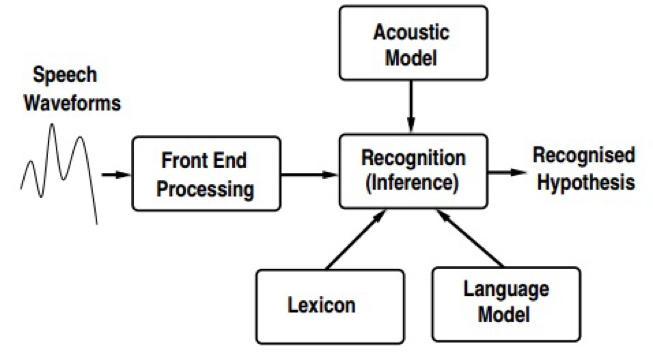
\includegraphics[width=4cm]{intro/ASR.png}
    \bicaption[fig:asr]{自动语音识别系统}{ASR structure}{Fig}{自动语音识别系统的结构}
  \end{minipage}     
\end{figure}

语音识别的第一阶段是压缩语音信号(逐帧)为声学特征向量的流, 称为观测值。提取的观测向量被设计成包含足够的信息以及足够紧凑来执行有效的语音识别。这一过程被称为前端处理或特征提取。从观测特征向量说开来,ASR系统可分为三个主要部分:词汇,语言模型和声学模型。词汇或者称为词典,用于映射出在声学模型中的子字单元到词汇与语言模型中的实际单词。语言模型代表了已说出句子的当地句法和语义信息。它对每个单词序列都分配了个可能性。声学模型,通常是语音研究者们最感兴趣的,映射了语音观测值到子字单元。 GMM-HMM框架一直是ASR框架的最先进技术,直到最近深度神经网络(DNN)被引入到ASR系统中。计划中的深度神经网络HMM(DNN-HMM)相比于最先进的GMM-HMM来说在两种任务上都取得了显著进步,音素识别[1]和大词汇连续语音识别(LVCSR)[2]任务。它使用一个深度神经网络(DNN)来计算聚类后状态并将其转换为可用于HMM的状态和条件似然概率。

深度神经网络(DNN)比起浅层的神经网络有更强大的模拟/建模能力。但是, 它也更有可能因为正常初始化策略和反向传播(BP)优化而陷入局部的最优。RBM(受限玻耳兹曼机)的预训练[1]或区别预训练[3]被提出来用作初始化权重矩阵到一个更好的起点,这使BP微调过程更容易,而且收敛更快速。最近,文献[4][5]介绍了更先进的训练标准,它们已被应用于得到更精确的模型。除了混合框架,DNN也可以用于获得更完善的瓶颈特征[6],以训练GMM-HMM系统并已经实现了与DNN相匹配的性能。

随着自动化语音识别的不断优化和发展,在识别中扮演重要角色的语言模型的研究同样得到迅速发展。语言模型在语音识别中扮演的角色是将声学模型识别得到的读音转化为最为合理的文字。用量化的值来衡量众多可能的文字搭配,语言模型的作用和用法就体现在这。


\section{语言模型的相关研究}
在20世纪90年代,最初的语言模型N-gram语言模型开始被提出。N-gram语言模型原理简单,仅需要掌握简单的概率论基础知识和极大似然概率就能实现,而且速度很快,对于当时的计算机硬件条件来说适用性很高,很快就被广泛接受和应用开来。这样一来,很多缺点和不足也就暴露出来,比如当训练数据不足的情况下很容易出现很多单词的预测概率为0,于是就有很多学者提出各种平滑算法来解决语料稀疏的问题[7][8][9],例如Kneser-Ney Smoothing等,除了这些诉算法,在N-gram的训练形式和语料的预处理方面专家们也是下足了功夫,例如Cache-based N-gram Model用缓存记录历史信息,Class-based N-gram Model将单词进行分类处理以及Topic-based N-gram Model在训练单词的时候为其配备topic附加信息以达到更好的训练等。
随着21世纪深度学习方法被证实可用,神经网络算法开始被用于自动语音识别和语言模型的学习当中。开始的DNN算法由于无法记录较长的历史信息而不适用于语言模型,因为语言是具有前后文连贯性的。接着随着RNN语言模型的提出,发现具有环状结构能够记录所有的历史信息的RNN网络非常适用于语言模型。

开始的RNN语言模型是一个词一个词的训练,但是速度太慢是它的弊端,后来学者将优化N-gram语言模型的思想扩展到语言模型上,提出一系列优化RNN语言模型的算法。Class based RNNLM被提出,它的思想同N-gram一样,对训练单词进行分类训练,能够有效的提高训练速度,并且对于丰富多彩的语言来说,那些出现概率偏小的词汇在预测中容易导致概率为0的问题得到了平滑。接着有人提出加入长短时间记忆的神经网络语言模型来学习那些有很长一段时间滞后并且滞后时间的长短未知的句子,它同样是RNNLM的一种扩展形式,通过分割记忆块的形式控制误差的传递时机,训练得到语言模型的性能相比传统RNNLM具有一定提升。除此之外,加入前后文相关信息的RNN语言模型于近年被Mikolov提出,它在训练当前单词的时候加入前后文块,并为词性加入话题信息,结合话题模型一起进行训练,形成一个受话题制约的RNNLM,可以有效避免数据在不同类型的数据子集上训练话题模型导致的数据分裂。多任务学习同样受到了很大的关注,其主要思想是在训练语言模型时加入其它的任务混合训练,共用一定数量的隐藏层或参数矩阵,达到相互促进相互制约的作用。

从语言模型训练速度的方向考虑,以前的语言模型不能同声学模型一样进行minibatch训练(nimibatch即是把训练数据分批输入到神经网络中进行学习),因为语言模型的识别往往和前后文以及历史信息关系密切,然而去年有学者提出可以换种方式考虑minibatch,同时读入很多句子,在不同的没有关联的句子中选取不同的单词进行minibatch输出,则不会影响学习相关性的情况下还能对速度有所提升。另外多核并行学习,利用GPU和Intel函数库进行训练等方法逐渐被用于语言模型训练上。

\section{本文的研究内容及研究意义}
本课题主要研究多视角融合的神经网络语言模型,即在循环神经网络的基础上加入多视角融合信息,将各信息的特征向量和词向量一同加入语言模型中训练,以提高语言模型的性能。

因为语言本身具有一些约束特性,如单词的识别会依赖于词性的连接规律、话题的约束和场景的区分等。本文首先将数据集预处理,分别通过对应的算法得到数据对应的词性、话题和场景等不同的信息,并进行标注得到新的数据集。然后,以词为单位对带标记的数据进行解析,得到其词向量和对应信息的特征向量。最后将这些向量一同作为RNNLM的输入层进行训练。

经过本文的研究和通过多组对比实验可以发现,多视角融合的RNNLM相比于传统的RNNLM在各类数据上均有8%左右的perplexity性能提升,在ASR的实验中也表现出了显著提高。证实了多视角融合的算法在神经网络的学习中切实可行,训练得到的语言模型不但模型本身性能有提高,在应用中例如ASR也表象良好,并且针对中文语料效果明显。并且在提高性能的情况下不增加时间复杂度,在不提高训练时间的情况下提升性能。无论在研究还是应用层面上都意义非凡。


\section{论文结构}
本论文剩下的部分是这样组织内容的:
第二章主要介绍什么是语言模型,语言模型的作用,以及各类语言模型。首先介绍最基本的,出现最早也是应用范围最广的N-gram语言模型,它是非神经网络语言模型,本文着重从它的定义和结构,以及数学原理等方面进行分析,然后简单介绍它的优化和变形,在第五章N-gram开源工具srilm将会作为实验对比工具出现。然后引入本文的重点——神经网络语言模型,主要从概念上介绍神经网络的定义,以及基本的三类神经网络语言模型:深度神经网络、循环神经网络、和长短时间记忆神经网络,同时引入神经元的基本结构。

第三章是深入探讨循环神经网络语言模型(RNNLM)。由于本文的研究内容“多视角融合神经网络语言模型”是基于RNNLM进行的优化和扩展,因此RNNLM的数学原理和训练步骤对本文的研究至关重要。本章首先介绍RNNLM的结构计算神经元的数学原理,然后引入RNNLM的完整训练步骤,接着着重推导RNNLM的训练中最重要的一部分——基于时间的反向传播(BPTT),它是RNNLM训练过程的精华所在。最后简单介绍RNNLM的几个相关开源工具,其中XRNN将会在第五章作为实验对比工具出现。

第四章是本文最重要的部分,全面介绍多视角融合的神经网络语言模型(Multiview-RNNLM)。首先介绍本研究用到的三种视角:词性、话题、场景,以及他们对语言模型的训练有何积极作用,然后分别提出各自的特征向量提取方法。接着提出Multiview-RNNLM如何的模型结构,以及如何加入这些特征向量一起训练的原理和数学支持。
第五章是实验部分,首先引入实验的基础知识,然后提出实验的设计和流程,同时介绍实验的平台、数据选取等一系列相关内容。最后对所有的实验数据进行展示、对比、分析,得出结论并进行总结。


